\section{Digitale Regelungstechnik (Grundlagen)}

\subsection{Arbeitsweise realer Abtastsysteme}
\begin{tcolorbox}
\boxtitle{Signalpfad eines digitalen Regelkreises}
Im digitalen Regelkreis werden zeitkontinuierliche Signale periodisch mit der Abtastzeit $T_A$ (bzw. $\omega_A = 2\pi/T_A$) abgetastet:
\begin{enumerate}
  \item \textbf{Anti-Aliasing-Filter:} Analoges Tiefpassfilter vor der Abtastung zur Einhaltung des Shannon-Theorems ($f_g < f_A/2$).
  \item \textbf{Abtastglied (Sampler):} Entnimmt äquidistante Abtastwerte $e(k T_A)$.
  \item \textbf{Analog-Digital-Wandler (ADW):} Wandelt die Spannung in ein $N$-Bit-Wort.
  \[
  \text{Auflösung: } LSB = \frac{U_{\text{FS}}}{2^N - 1} \approx \frac{U_{\text{FS}}}{2^N}
  \]
  Quantisierungsrauschen: maximaler Fehler $\pm \frac{1}{2} LSB$.
  \item \textbf{Digitalrechner / Mikrocontroller:} Berechnet den Regelalgorithmus in einer festen Interrupt-Zeitscheibe $T_A$.
  \item \textbf{Halteglied nullter Ordnung (ZOH):} Hält den berechneten Stellwert $u(k T_A)$ über das Intervall $T_A$ konstant:
  \[
  g_{h0}(t) = \sigma(t) - \sigma(t - T_A) \implies G_{h0}(s) = \frac{1 - e^{-s T_A}}{s}
  \]
\end{enumerate}
\end{tcolorbox}

\begin{center}
  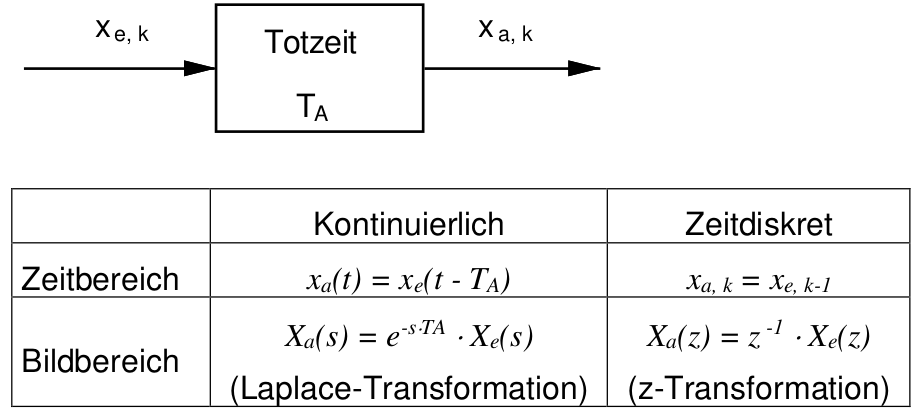
\includegraphics[width=\columnwidth]{images/abtastung_zeit.png}
\end{center}

\subsection{Die $z$-Transformation}
\begin{tcolorbox}
\boxtitle{Definition}
Für ein kausales diskretes Zeitsignal $\{f_k\} = \{f(k T_A)\}$ mit $f_k = 0$ für $k < 0$:
\[
F(z) = \mathcal{Z}\{f_k\} = \sum_{k=0}^\infty f_k \cdot z^{-k} \quad \text{mit } z = e^{s T_A}
\]
$z^{-1}$ entspricht im Zeitbereich einer Verzögerung um genau einen Abtastschritt $T_A$.
\end{tcolorbox}

\begin{tcolorbox}
\boxtitle{Korrespondenztabelle der $z$-Transformation}
\small
\begin{tabularx}{\columnwidth}{l X l}
\toprule
\textbf{Signal $f(t)$} & \textbf{Folge $f_k$} & \textbf{$z$-Transformierte $F(z)$} \\
\midrule
Impuls $\delta(t)$ & $\delta_k = (1, 0, 0, \dots)$ & $1$ \\[2pt]
Sprung $\sigma(t)$ & $\sigma_k = (1, 1, 1, \dots)$ & $\frac{z}{z-1}$ \\[3pt]
Rampe $t$ & $k \cdot T_A$ & $\frac{T_A z}{(z-1)^2}$ \\[3pt]
Parabel $t^2$ & $k^2 T_A^2$ & $\frac{T_A^2 z (z+1)}{(z-1)^3}$ \\[3pt]
Exp-Funktion $e^{-at}$ & $e^{-a k T_A}$ & $\frac{z}{z - e^{-a T_A}}$ \\[3pt]
$1 - e^{-at}$ & $1 - e^{-a k T_A}$ & $\frac{z (1 - e^{-a T_A})}{(z-1)(z - e^{-a T_A})}$ \\[3pt]
$t \cdot e^{-at}$ & $k T_A e^{-a k T_A}$ & $\frac{T_A z e^{-a T_A}}{(z - e^{-a T_A})^2}$ \\[3pt]
$\sin(\omega t)$ & $\sin(\omega k T_A)$ & $\frac{z \sin(\omega T_A)}{z^2 - 2z\cos(\omega T_A) + 1}$ \\[3pt]
$\cos(\omega t)$ & $\cos(\omega k T_A)$ & $\frac{z (z - \cos(\omega T_A))}{z^2 - 2z\cos(\omega T_A) + 1}$ \\[3pt]
$e^{-at}\sin(\omega t)$ & $e^{-ak T_A}\sin(\omega k T_A)$ & $\frac{z e^{-aT_A} \sin(\omega T_A)}{z^2 - 2z e^{-aT_A}\cos(\omega T_A) + e^{-2aT_A}}$ \\[3pt]
$e^{-at}\cos(\omega t)$ & $e^{-ak T_A}\cos(\omega k T_A)$ & $\frac{z (z - e^{-aT_A}\cos(\omega T_A))}{z^2 - 2z e^{-aT_A}\cos(\omega T_A) + e^{-2aT_A}}$ \\
\bottomrule
\end{tabularx}
\end{tcolorbox}

\begin{tcolorbox}
\boxtitle{Rechenregeln der $z$-Transformation}
\small
\begin{itemize}
  \item \textbf{Linearität:} $\mathcal{Z}\{a f_{1k} + b f_{2k}\} = a F_1(z) + b F_2(z)$
  \item \textbf{Rechtsverschiebung (Verzögerung um $n$ Schritte):}
  \[
  \mathcal{Z}\{f_{k-n}\} = z^{-n} \cdot F(z) \quad (\text{für } f_k = 0 \text{ bei } k < 0)
  \]
  \item \textbf{Linksverschiebung (Vorauseilung):}
  \[
  \mathcal{Z}\{f_{k+n}\} = z^n \left[ F(z) - \sum_{i=0}^{n-1} f_i z^{-i} \right]
  \]
  \item \textbf{Rückwärtsdifferenz:}
  \[
  \mathcal{Z}\{f_k - f_{k-1}\} = \frac{z-1}{z} F(z) - f_{-1}
  \]
  \item \textbf{Vorwärtsdifferenz:}
  \[
  \mathcal{Z}\{f_{k+1} - f_k\} = (z-1) F(z) - f_0 z
  \]
  \item \textbf{Dämpfungssatz:}
  \[
  \mathcal{Z}\{f_k \cdot e^{-a k T_A}\} = F(z \cdot e^{a T_A})
  \]
  \item \textbf{Summensatz:}
  \[
  \mathcal{Z}\left\{ \sum_{\nu=0}^k f_\nu \right\} = \frac{z}{z-1} \cdot F(z)
  \]
  \item \textbf{Differentiation im Bildbereich:}
  \[
  \mathcal{Z}\{k \cdot f_k\} = -z \cdot \frac{d F(z)}{dz}
  \]
  \item \textbf{Faltungssatz:}
  \[
  \mathcal{Z}\{f_k * g_k\} = \mathcal{Z}\left\{ \sum_{\nu=0}^k f_\nu g_{k-\nu} \right\} = F(z) \cdot G(z)
  \]
  \item \textbf{Anfangswertsatz:}
  \[
  f_0 = f(t \to 0) = \lim_{z \to \infty} F(z)
  \]
  \item \textbf{Endwertsatz:}
  \[
  f_\infty = \lim_{k \to \infty} f_k = \lim_{z \to 1} (z - 1) \cdot F(z)
  \]
  (Voraussetzung: Alle Pole von $(z-1)F(z)$ liegen strikt innerhalb des Einheitskreises).
\end{itemize}
\end{tcolorbox}

\subsection{Stabilität im $z$-Bereich}
\begin{tcolorbox}
Ein zeitdiskretes LTI-System mit der $z$-Übertragungsfunktion $F(z)$ ist genau dann \textbf{BIBO-stabil}, wenn alle Pole $z_{P,i}$ von $F(z)$ \textbf{strikt innerhalb des Einheitskreises} der komplexen $z$-Ebene liegen:
\[
|z_{P,i}| < 1 \quad \forall i = 1, \dots, n
\]
\textbf{Abbildung der $s$-Ebene in die $z$-Ebene:}
Mit $s = \sigma + j\omega$ und $z = e^{s T_A}$:
\[
z = e^{(\sigma + j\omega) T_A} = e^{\sigma T_A} \cdot e^{j \omega T_A} \implies |z| = e^{\sigma T_A}, \quad \angle z = \omega T_A
\]
\begin{itemize}
  \item $\sigma < 0$ (linke $s$-Halbebene, stabil) $\implies |z| < 1$ (Inneres des Einheitskreises).
  \item $\sigma = 0$ (Imaginärachse, Stabilitätsgrenze) $\implies |z| = 1$ (Einheitskreislinie).
  \item $\sigma > 0$ (rechte $s$-Halbebene, instabil) $\implies |z| > 1$ (Äußeres des Einheitskreises).
  \item $0 < z < 1$ (positive reelle Achse): Rein aperiodisches Verhalten ($D \ge 1$, kein Überschwingen).
  \item $-1 < z < 0$ (negative reelle Achse): Oszillation mit der halben Abtastfrequenz $\omega = \frac{\pi}{T_A} = \frac{\omega_A}{2}$ (Nyquist-Grenze, da $(-1)^k$ alterniert).
  \item $z = 0$ (Ursprung): Vollkommene Dämpfung / Deadbeat (Antwort klingt in endlich vielen Schritten exakt ab).
  \item $z = 1$: Integrator ($s = 0$).
\end{itemize}
\end{tcolorbox}

\subsection{Näherungsverfahren zur Transformation $s \to z$}
\begin{tcolorbox}
Da der exakte Zusammenhang $z = e^{s T_A}$ für gebrochen rationale Funktionen nicht rational ist, verwendet man Näherungen:

\textbf{1. Rückwärtsdifferenzenquotient:}
\[
s \approx \frac{1 - z^{-1}}{T_A} = \frac{z - 1}{T_A \cdot z}
\]
Ersetzung: $F(z) = F(s)\big|_{s = \frac{z-1}{T_A z}}$.
Stabile $s$-Systeme bleiben immer stabil. Allerdings können instabile $s$-Pole fälschlich in den Einheitskreis abgebildet werden.

\textbf{2. Vorwärtsdifferenzenquotient (Euler):}
\[
s \approx \frac{z - 1}{T_A}
\]
Ersetzung: $F(z) = F(s)\big|_{s = \frac{z-1}{T_A}}$.
Sehr einfach zu berechnen. Nachteil: Stabile $s$-Systeme können im $z$-Bereich instabil werden!

\textbf{3. Tustinsche Formel (Bilineartransformation):}
\[
s \approx \frac{2}{T_A} \cdot \frac{z - 1}{z + 1}
\]
Bildet die gesamte linke $s$-Halbebene bijektiv auf das Innere des Einheitskreises ab. Stabilität bleibt exakt erhalten.
\textbf{Frequenzverzerrung (Prewarping):}
\[
\omega_w = \frac{2}{T_A} \tan\left( \frac{\omega T_A}{2} \right)
\]
\end{tcolorbox}

\subsection{Rechenalgorithmus aus $F(z)$}
\begin{tcolorbox}
\boxtitle{Vorgehensweise zur Bestimmung der Differenzengleichung}
Gegeben ist die $z$-Übertragungsfunktion $F(z) = \frac{X_a(z)}{X_e(z)}$:
\begin{enumerate}
  \item Zähler und Nenner durch die höchste Potenz von $z$ teilen, sodass nur Terme $z^0, z^{-1}, z^{-2}, \dots$ verbleiben.
  \[
  F(z) = \frac{b_0 + b_1 z^{-1} + \dots + b_m z^{-m}}{a_0 + a_1 z^{-1} + \dots + a_n z^{-n}}
  \]
  \item Ausmultiplizieren:
  \[
  X_a(z) \cdot \sum a_i z^{-i} = X_e(z) \cdot \sum b_i z^{-i}
  \]
  \item Rücktransformation in den Zeitbereich ($z^{-i} \leftrightarrow$ Verzögerung um $i$ Abtastschritte):
  \[
  a_0 x_{a,k} + a_1 x_{a,k-1} + \dots = b_0 x_{e,k} + b_1 x_{e,k-1} + \dots
  \]
  \item Auflösen nach dem aktuellen Stellwert $x_{a,k}$:
  \[
  x_{a,k} = \frac{1}{a_0} \left[ \sum_{i=0}^m b_i x_{e,k-i} - \sum_{j=1}^n a_j x_{a,k-j} \right]
  \]
\end{enumerate}
\textbf{Beispiel:}
\[
F(z) = \frac{2z + 4}{8z - 5} = \frac{2 + 4 z^{-1}}{8 - 5 z^{-1}}
\]
\[
8 x_{a,k} - 5 x_{a,k-1} = 2 x_{e,k} + 4 x_{e,k-1}
\]
\[
\implies x_{a,k} = 0{,}25 \cdot x_{e,k} + 0{,}50 \cdot x_{e,k-1} + 0{,}625 \cdot x_{a,k-1}
\]
\end{tcolorbox}

\begin{tcolorbox}
\boxtitle{Implementierung in Programmcode (C)}
\begin{lstlisting}
while (1) {
    wait_timerinterrupt(TA); // Abtastzeit warten
    
    // Alte Werte weiterschieben
    xaalt1 = xa;
    xealt1 = xe;
    
    // Eingangswert einlesen
    input(xe);
    
    // Differenzengleichung berechnen
    xa = 0.25 * xe + 0.50 * xealt1 + 0.625 * xaalt1;
    
    // Stellwert ausgeben
    output(xa);
}
\end{lstlisting}
\end{tcolorbox}

\subsection{Kausalität \& Signalflussplan im Diskreten}
\begin{tcolorbox}
\textbf{Kausalitätsbedingung:}\\[2pt]
Ein diskretes System ist als physikalischer Rechenalgorithmus genau dann realisierbar, wenn der Nennergrad mindestens so groß ist wie der Zählergrad:
\[
\deg(\text{Zähler}) \le \deg(\text{Nenner}) \iff m \le n
\]
\begin{itemize}
  \item $m < n$: Streng kausal (Ausgang hängt nur von vergangenen Eingängen ab, Verzögerung um $(n-m) T_A$).
  \item $m = n$: Kausal (Ausgang hängt auch vom aktuellen Eingang $x_{e,k}$ ab).
  \item $m > n$: Nicht kausal (erfordert zukünftige Werte $x_{e,k+1} \implies$ nicht echtzeitfähig!).
\end{itemize}
\end{tcolorbox}
